\subsubsection{MSVC: x86}

\lstinputlisting{patterns/04_scanf/2_global/ex2_MSVC.asm}

In questo caso la variabile \TT{x} è definita nel segmento \TT{\_DATA} e per essa non viene allocata alcuna memoria nello stack locale. Viene acceduta direttamente, non attraverso lo stack.
Le variabili globali non inizializzate non occupano spazio nel file eseguibile 
(che motivo ci sarebbe di allocare spazio per varibaili inizialmente settate a zero?), 
ma quanto qualcuno accede al loro indirizzo, l' \ac{OS} allocherà un bloco di zeri al loro posto \footnote{Questo è il modo in cui vunziona una \ac{VM} }.

Adesso assegnamo esplicitamente un valore alla variabile:

\lstinputlisting{patterns/04_scanf/2_global/default_value_EN.c}

Otteniamo:

\begin{lstlisting}
_DATA	SEGMENT
_x	DD	0aH

...
\end{lstlisting}

Vediamo qui un valore \TT{0xA} di tipo DWORD (DD sta per DWORD = 32 bit) per questa variabile.

Analizzando con \IDA il file .exe compilato, notiamo che la variabile \IT{x} è collocata all'inizio del segmento \TT{\_DATA}, e dopo di essa vediamo le stringhe testuali.

Analizzando l'eseguibile dell'esempio precedente con \IDA, vedremo qualcosa del genere dove il valore di \IT{x} non era stato impostato:

\begin{lstlisting}
.data:0040FA80 _x              dd ?                    ; DATA XREF: _main+10
.data:0040FA80                                         ; _main+22
.data:0040FA84 dword_40FA84    dd ?                    ; DATA XREF: _memset+1E
.data:0040FA84                                         ; unknown_libname_1+28
.data:0040FA88 dword_40FA88    dd ?                    ; DATA XREF: ___sbh_find_block+5
.data:0040FA88                                         ; ___sbh_free_block+2BC
.data:0040FA8C ; LPVOID lpMem
.data:0040FA8C lpMem           dd ?                    ; DATA XREF: ___sbh_find_block+B
.data:0040FA8C                                         ; ___sbh_free_block+2CA
.data:0040FA90 dword_40FA90    dd ?                    ; DATA XREF: _V6_HeapAlloc+13
.data:0040FA90                                         ; __calloc_impl+72
.data:0040FA94 dword_40FA94    dd ?                    ; DATA XREF: ___sbh_free_block+2FE
\end{lstlisting}

\TT{\_x} è contrassegnata con il simbolo \TT{?} insiema lresto delle variabili che non necessitano di essere inizializzate.
Ciò implica che dopo il caricamento del .exe in memoria, verrà allocato spazio riempito di zeri per tutte queste variabili.[\CNineNineStd 6.7.8p10].
Ma nel file .exe tutte le variabili non inizializzate non occupano alcuno spazio.
Questo risulta molto conveniente ad esempio nel caso di array molto grandi.

\EN{\clearpage
\subsection{MSVC: x86 + \olly}
\myindex{\olly}

Things are even simpler here:

\begin{figure}[H]
\centering
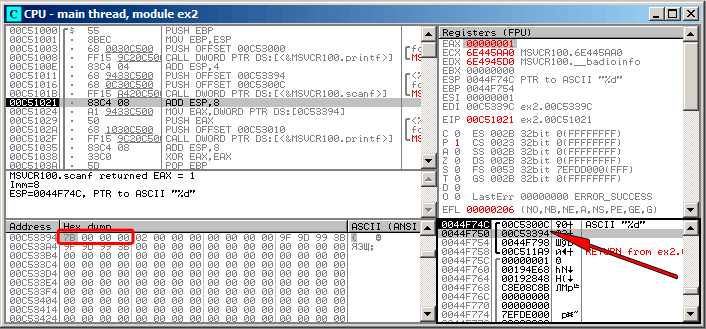
\includegraphics[scale=\FigScale]{patterns/04_scanf/2_global/ex2_olly_1.png}
\caption{\olly: after \scanf execution}
\label{fig:scanf_ex2_olly_1}
\end{figure}

The variable is located in the data segment.
After the \PUSH instruction (pushing the address of $x$) gets executed, 
the address appears in the stack window. Right-click on that row and select \q{Follow in dump}.
The variable will appear in the memory window on the left.
After we have entered 123 in the console, 
\TT{0x7B} appears in the memory window (see the highlighted screenshot regions).

But why is the first byte \TT{7B}?
Thinking logically, \TT{00 00 00 7B} should be
there.
The cause for this is referred as  \gls{endianness}, and x86 uses \IT{little-endian}.
This implies that the lowest byte is written first, and the highest written last.
Read more about it at: \myref{sec:endianness}.
Back to the example, the 32-bit value is loaded from this memory address into \EAX and passed to \printf.

The memory address of $x$ is \TT{0x00C53394}.

\clearpage
In \olly we can review the process memory map (Alt-M)
and we can see that this address is inside the \TT{.data} PE-segment of our program:

\begin{figure}[H]
\centering
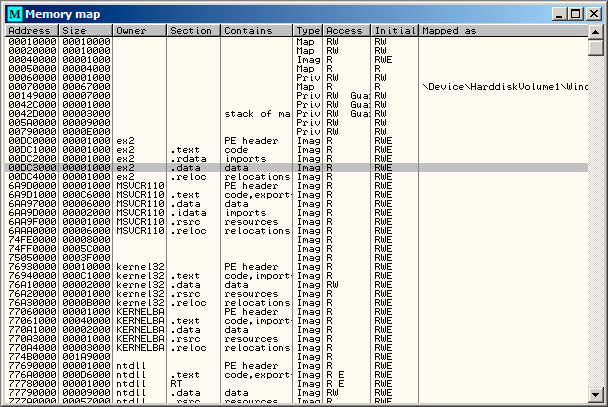
\includegraphics[scale=\FigScale]{patterns/04_scanf/2_global/ex2_olly_2.png}
\caption{\olly: process memory map}
\label{fig:scanf_ex2_olly_2}
\end{figure}

}
\RU{\clearpage
\subsectionold{MSVC: x86 + \olly}
\myindex{\olly}

Тут даже проще:

\begin{figure}[H]
\centering
\myincludegraphics{patterns/04_scanf/2_global/ex2_olly_1.png}
\caption{\olly: после исполнения \scanf}
\label{fig:scanf_ex2_olly_1}
\end{figure}

Переменная хранится в сегменте данных.
Кстати, после исполнения инструкции \PUSH (заталкивающей адрес $x$) адрес появится в стеке, 
и на этом элементе можно нажать правой кнопкой, выбрать \q{Follow in dump}.
И в окне памяти слева появится эта переменная.

После того как в консоли введем 123, здесь появится \TT{0x7B}.

Почему самый первый байт это \TT{7B}?
По логике вещей, здесь должно было бы быть \TT{00 00 00 7B}.
Это называется \gls{endianness}, и в x86 принят формат \IT{little-endian}.
Это означает, что в начале записывается самый младший байт, а заканчивается самым старшим байтом.
Больше об этом: \myref{sec:endianness}.

Позже из этого места в памяти 32-битное значение загружается в \EAX и передается в \printf.

Адрес переменной $x$ в памяти \TT{0x00C53394}.

\clearpage
В \olly{} мы можем посмотреть карту памяти процесса (Alt-M) и увидим, что этот адрес
внутри PE-сегмента \TT{.data} нашей программы:

\begin{figure}[H]
\centering
\myincludegraphics{patterns/04_scanf/2_global/ex2_olly_2.png}
\caption{\olly: карта памяти процесса}
\label{fig:scanf_ex2_olly_2}
\end{figure}
}
\ITA{\clearpage
\subsectionold{MSVC: x86 + \olly}
\myindex{\olly}

Il quadro qui è ancora più semplice:

\begin{figure}[H]
\centering
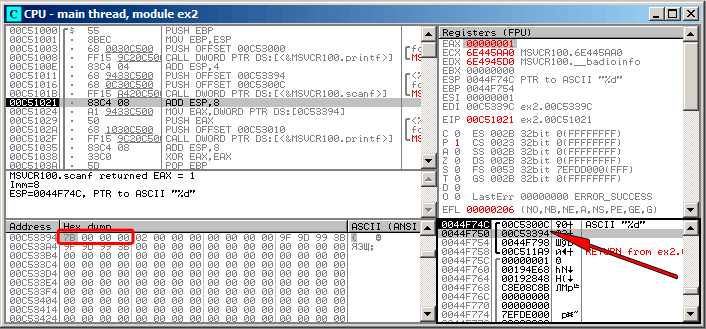
\includegraphics[scale=\FigScale]{patterns/04_scanf/2_global/ex2_olly_1.png}
\caption{\olly: after \scanf execution}
\label{fig:scanf_ex2_olly_1}
\end{figure}

La variabile è collocata nel data segment.
Dopo che l'istruzione \PUSH (che fa il push dell'indirizzo di $x$) viene eseguita, 
l'indirizzo appare nella finestra dello stack. Facciamo click destro su quella riga e selezioniamo \q{Follow in dump}.
La variabile apparirà nella finestra di memoria a sinistra.
Dopo aver inserito il valore 123 in console, 
\TT{0x7B} apparirà nella finestra della memoria (vedere regioni evidenziate nello screenshot).

Ma perchè il primo byte è \TT{7B}?
A rigor di logica, dovremmo trovare \TT{00 00 00 7B}.
La causa per cui troviamo invece \TT{7B} è detta \gls{endianness}, e x86 usa la convenzione \IT{little-endian}.
Ciò significa che il byte piu basso è scritto per primo, e quello più alto per ultimo.
Maggiori informazioni sono disponibili nella sezione: \myref{sec:endianness}.
Tornando all'esempio, il valore a 32-bit è caricato da questo indirizzo di memoria in \EAX e passato a \printf.

L'indirizzo in memoria di $x$ è \TT{0x00C53394}.

\clearpage
In \olly possiamo osservare la mappa di memoria di un processo  (process memory map, Alt-M)
e notare che questo indirizzo è dentro il segmento PE \TT{.data} del nostro programma:

\begin{figure}[H]
\centering
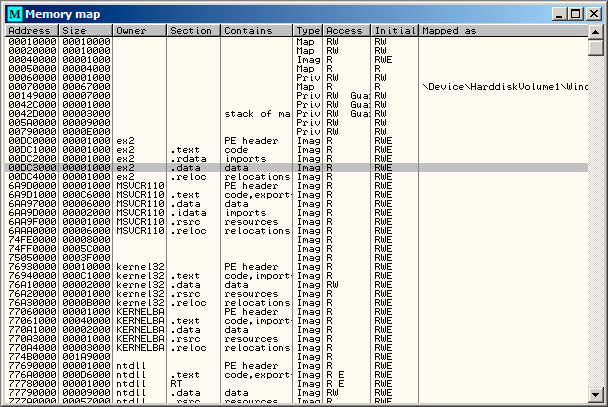
\includegraphics[scale=\FigScale]{patterns/04_scanf/2_global/ex2_olly_2.png}
\caption{\olly: process memory map}
\label{fig:scanf_ex2_olly_2}
\end{figure}

}


\subsubsection{GCC: x86}

\myindex{ELF}
La situazione in Linux è pressoché identica, con la differenza che le variabili non inizializzate sono collocate nel segmento \TT{\_bss}. 
In un file \ac{ELF} questo segmento ha i seguenti attributi:

\begin{lstlisting}
; Segment type: Uninitialized
; Segment permissions: Read/Write
\end{lstlisting}

Se invece si inizializza la variabile con un qualunque valore, es. 10, 
sarà collocata nel segmento \TT{\_data}, che ha i seguenti attributi:

\begin{lstlisting}
; Segment type: Pure data
; Segment permissions: Read/Write
\end{lstlisting}

\subsubsection{MSVC: x64}

\lstinputlisting[caption=MSVC 2012 x64]{patterns/04_scanf/2_global/ex2_MSVC_x64_EN.asm}

Il codice è pressoché identico a quello in x86.
Si noti che l'indirizzo della variabile $x$ è passato a \TT{scanf()} usando un'istruzione \LEA ,
mentre il valore della variabile è passato alla seconda \printf usando un'istruzione \MOV.
\TT{DWORD PTR}--- è parte del linguaggio assembly (non ha a che vedere con il codice macchina),
indica che la dimensione del dato della variabile è 32-bit e l'istruzione \MOV deve essere codificata in accordo alla dimensione.

